%====================================================================
%   SECTION 3 — PAIRS TRADING WITH THE BASELINE
%====================================================================

\section{Pairs trading with the baseline}\label{sec:pairsbaseline}

This section defines the baseline strategy as a self-contained pairs-trading rule \parencite{gatev2006pairs,vidyamurthy2004pairs}. The regime-aware extensions of Section~\ref{sec:regimemodels} keep this rule's entry direction and only modify when it is allowed to trade.

\subsection{Cointegration spread}\label{sec:spread}

Two non-stationary log-price series $\log P_t^{\mathrm{mid},\,A}$ and $\log P_t^{\mathrm{mid},\,B}$ are cointegrated if some linear combination is stationary \parencite{engle1987cointegration}:
\begin{equation}\label{eq:spreaddef}
    S_t \;=\; \log P_t^{\mathrm{mid},\,A} \;-\; \beta\,\log P_t^{\mathrm{mid},\,B}.
\end{equation}
The hedge ratio $\beta$ is estimated by the Engle--Granger two-step procedure: OLS regression of $\log P^{\mathrm{mid},\,A}$ on $\log P^{\mathrm{mid},\,B}$, with stationarity of the residuals verified by an Augmented Dickey--Fuller test \parencite{dickey1979distribution,said1984testing}. High-frequency FX is not globally cointegrated: $\beta$ drifts with liquidity, session structure, and pair-specific shocks. I therefore estimate $\beta_t$ by rolling OLS with window $W_\beta$. Writing $x_s = \log P_s^{\mathrm{mid},\,B}$, $y_s = \log P_s^{\mathrm{mid},\,A}$, and $\mathcal{W}_t = \{t-W_\beta+1,\ldots,t\}$ with window means $\bar x_t, \bar y_t$,
\begin{equation}\label{eq:rollingbeta}
    \beta_t \;=\; \frac{\sum_{s \in \mathcal{W}_t}(x_s - \bar x_t)(y_s - \bar y_t)}{\sum_{s \in \mathcal{W}_t}(x_s - \bar x_t)^{2}},
    \qquad
    \alpha_t \;=\; \bar y_t \;-\; \beta_t\, \bar x_t.
\end{equation}
The cointegration spread and its associated return are
\begin{equation}\label{eq:rollingspreadret}
\begin{aligned}
    S_t \;&=\; \log P_t^{\mathrm{mid},\,A} \;-\; \beta_t \log P_t^{\mathrm{mid},\,B} \;-\; \alpha_t,\\[2pt]
    \Delta S_t \;&=\; r_t^{A} \;-\; \beta_{t-1}\, r_t^{B},
\end{aligned}
\end{equation}
with bar log-returns $r_t^{i} = \log P_t^{\mathrm{mid},\,i} - \log P_{t-1}^{\mathrm{mid},\,i}$. The lag $\beta_{t-1}$ ensures the hedge ratio is observable when the return is realised.

\subsection{The rolling \texorpdfstring{$z$-score}{z-score} and the baseline rule}\label{sec:zscore}

The baseline reads $S_t$ through a rolling $z$-score over a window of length $W_z$,
\begin{equation}\label{eq:zscore}
    Z_t \;=\; \frac{S_t - \mu_t^{S}}{\sigma_t^{S}},
\end{equation}
with rolling mean and variance
\begin{equation*}
    \mu_t^{S} \;=\; \frac{1}{W_z}\sum_{s=t-W_z+1}^{t} S_s,
    \qquad
    \bigl(\sigma_t^{S}\bigr)^{2} \;=\; \frac{1}{W_z}\sum_{s=t-W_z+1}^{t}\bigl(S_s - \mu_t^{S}\bigr)^{2}.
\end{equation*}
With entry threshold $z_q$ and exit threshold $z_x$, the position $\pi_t \in \{-1,0,+1\}$ is updated by
\begin{equation}\label{eq:baselinerule}
    \pi_t \;=\;
    \begin{cases}
        +1 & \pi_{t-1}=0,\; Z_t < -z_q, \\
        -1 & \pi_{t-1}=0,\; Z_t > +z_q, \\
        \phantom{+}0 & \pi_{t-1} \neq 0,\; |Z_t| \leq z_x, \\
        \pi_{t-1} & \text{otherwise.}
    \end{cases}
\end{equation}
A long-spread position is opened when $S_t$ is sufficiently below its rolling mean and closed when it returns toward zero; the short rule is symmetric \parencite{gatev2006pairs}. For every unit of leg $A$ I trade $\hat{\beta}$ units of leg $B$, so the resulting portfolio is exposed to the relative move between the two legs rather than to FX direction \parencite{vidyamurthy2004pairs}. Figure~\ref{fig:longshort} illustrates the bookkeeping of a single round-trip on a representative pair.

\begin{figure}[H]
    \centering
    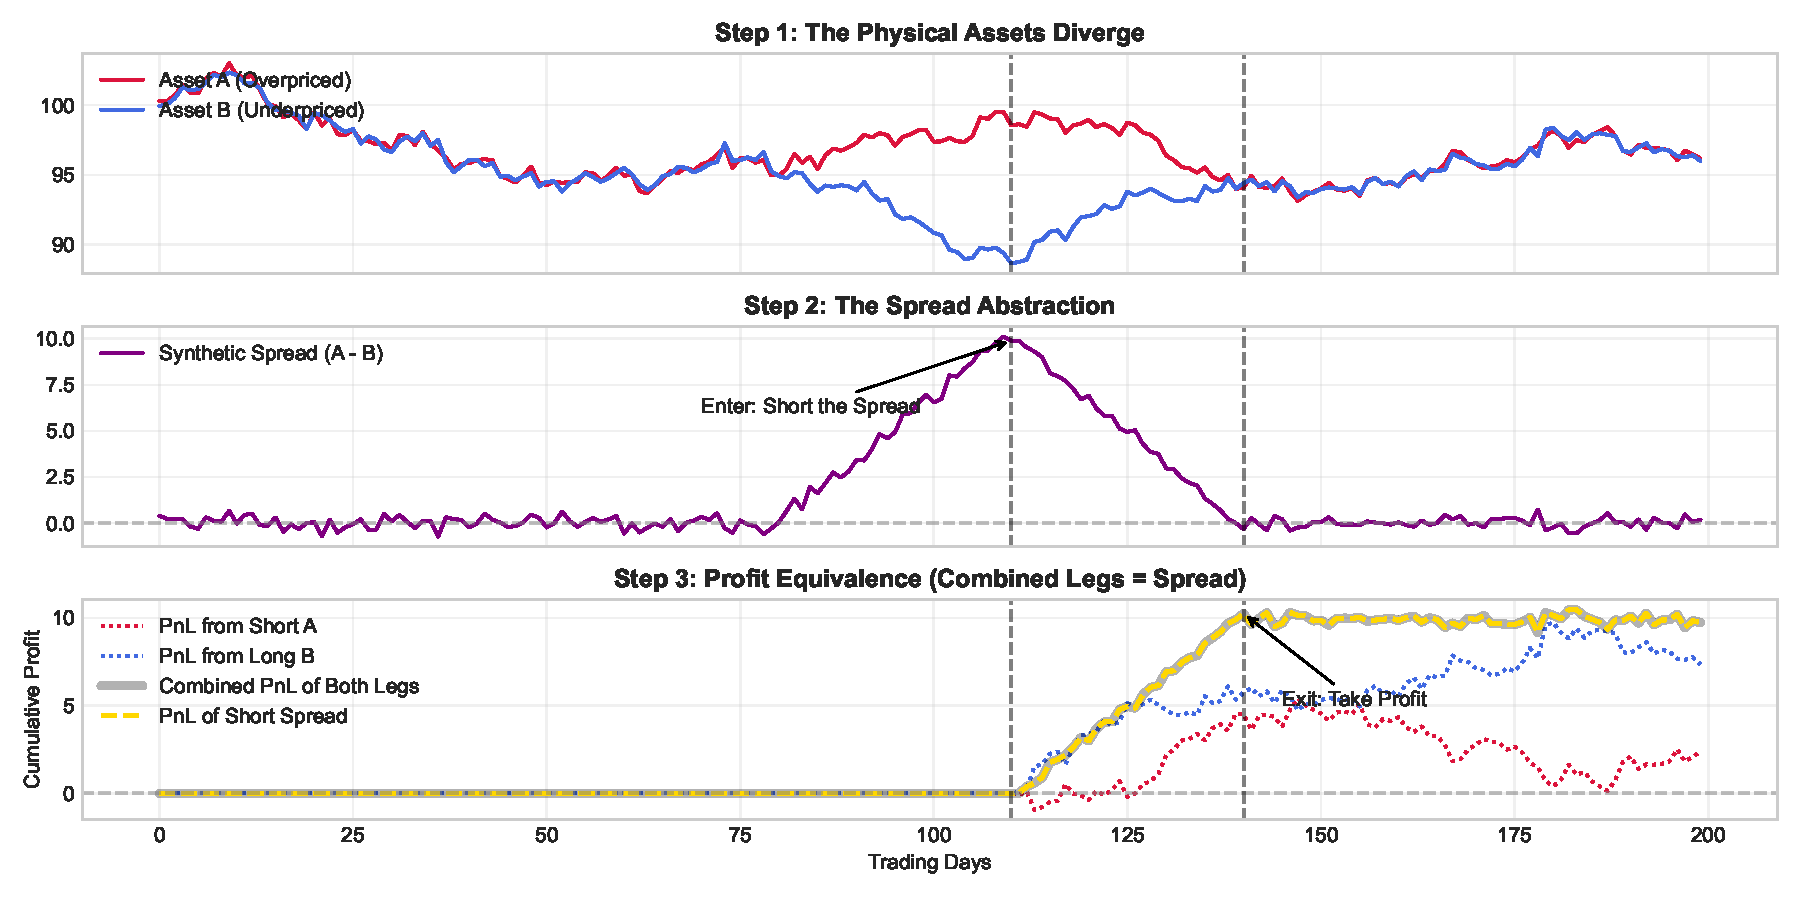
\includegraphics[width=\linewidth]{plots/long-short.pdf}
    \caption{Mechanics of a single pairs-trade. Top: the price path of each leg over the trade window. Bottom: the combined long/short portfolio, which is constructed to be exposed only to the relative move between the two legs and is approximately neutral to the common FX direction. The position is entered when the spread is far from its rolling mean (in $z$-score units) and closed as the spread reverts.}
    \label{fig:longshort}
\end{figure}

A do-nothing reference $\pi_t^{\mathrm{BH}} = +1$ for every $t$ (Buy \& Hold) earns $\Delta S_t$ at each step, pays no transaction costs, and provides a passive drift benchmark.

\subsection{Why the baseline is not enough}\label{sec:baselinelimits}

The baseline assumes $S_t$ is governed by a single stationary process, so that fixed $(z_q, z_x)$ correctly characterise ``far from equilibrium'' for every $t$. Two empirical features of FX tick data violate this assumption: (i) squared spread returns exhibit strong positive autocorrelation, consistent with conditional heteroskedasticity \parencite{engle1982arch,bollerslev1986garch,cont2001empirical}; and (ii) a spread that mean-reverts quickly in quiet periods may drift directionally for hundreds of bars during news-driven or one-sided-flow episodes \parencite{hasbrouck2007microstructure}. The fixed-threshold rule has no mechanism to distinguish these cases. This motivates the regime-aware extensions below.